%% Journal of Open Research Software Latex template -- Created By Stephen Bonner and John Brennan, Durham Universtiy, UK.
%\PassOptionsToPackage{xcolor}{dvipsnames}
\documentclass{jors}
\usepackage[author={Lyndon}]{pdfcomment}


\usepackage{listings}


\lstdefinelanguage{Julia}%%% Julia definition (c) 2014 Jubobs
{morekeywords={abstract,begin, break,case,catch,const,continue,do,else,elseif,%
		end,export,false,for,function,immutable,import,importall,if,in,%
		macro,module,otherwise,quote,return,switch,true,try,type,typealias,%
		using,while},%
	sensitive=true,%
	alsoother={$},%$ fix sybtaxhighligh
	morecomment=[l]\#,%
	morecomment=[n]{\#=}{=\#},%
	morestring=[s]{"}{"},%
	morestring=[m]{'}{'},%
}[keywords,comments,strings]%

\lstset{%
	language         = Julia,
	basicstyle       = \ttfamily,
	keywordstyle     = \bfseries\color{blue},
	stringstyle      = \color{magenta},
	commentstyle     = \color{green!50!black},
	showstringspaces = false,
}

%%%%%%%%%%%
%Graphics
\usepackage{graphicx}
\usepackage{tikz}
\usetikzlibrary{positioning,arrows,shapes}
\tikzset{
	every picture/.style={/utils/exec={\sffamily}},
	every matrix/.style={ampersand replacement=\&, rounded corners=10pt},
}
%%%%%%%%%%%%%%%%%

\usepackage[backend=bibtex, url=false,
style=authoryear-ibid 
]{biblatex}

\bibliography{master}
%%%%%%%%%%%%%%%%%%%


\newcommand{\datadep}[1]{\texttt{datadep"{}#1"{}}}

%%%%%%%%%%%%%%


%% Set the header information
\pagestyle{fancy}
\definecolor{mygray}{gray}{0.6}
\renewcommand\headrule{}
\rhead{\footnotesize 3}
\rhead{\textcolor{gray}{{DataDeps.jl -- Repeatable Data Setup For Reproducible Data and Computational Science}}}


%opening

\title{{DataDeps.jl -- Reproducible Data Setup For Repeatable Data and Computational Science}}
\author{}

\usepackage{cleveref}
\begin{document}

\maketitle

\begin{abstract}
We present a framework DataDeps.jl for the reproducible handling of static datasets to enhance the repeatability of software scripts used in the data and computational sciences.
DataDeps.jl automates the data setup part of running software accompanies a paper to replicate a result.
This step is commonly done manually, which expends time and allows for confusion.
It normally requires the user to follow instructions about how to download and extract the data, and how the script is to be informed of the data's location.
By automating this step it become to validate the scientific conclusions by executing the scripts.
It also simplifies extending such research software requiring the data via traditional means of a software dependency, and the later extension software does not have to worry about including even more complicated instructions about setting up the data for the software it depends upon.
DataDeps.jl makes it easier to rerun another authors code in a new environment.
\end{abstract}

\textbf{Keywords:} Julia; data; data management;  data dependencies; reproducible science; downloading; computational environment setup; continuous integration; software practices.


\rule{\textwidth}{1pt}


\begin{figure}
\resizebox{\textwidth}{!}{%
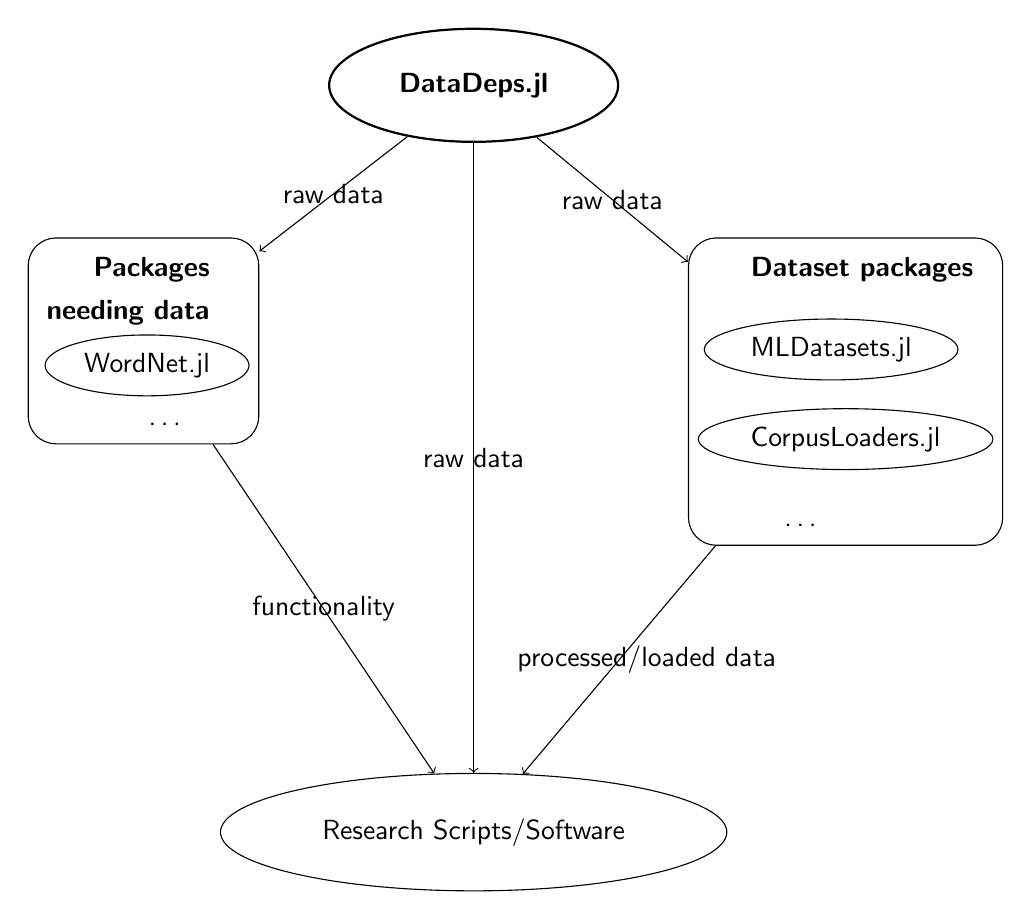
\begin{tikzpicture}[]
	\node[ellipse, thick, draw, inner sep = 10] (datadeps) {\textbf{DataDeps.jl}};
	\node[matrix, below right = 2 of datadeps, draw, column sep=15, row sep=10] (datasetpackages) {
		\node{\textbf{Dataset packages}}; \\
		\node[draw,ellipse]{MLDatasets.jl};\\
		\node[draw,ellipse]{CorpusLoaders.jl}; \\
		\node{\phantom{M} \ldots \phantom{M}};\\
	};
	\node[matrix, below left = 2 of datadeps, draw, column sep=15] (packages) {
		\node{\textbf{Packages}}; \\
		\node{\textbf{needing data}}; \\
		\node[draw,ellipse]{WordNet.jl}; \\
		\node{\phantom{M} \ldots \phantom{M}};\\
	};
	\node[ellipse, draw, inner sep = 10, below = 8 of datadeps] (researchcode) {Research Scripts/Software};
	
	\path[->,draw] (datadeps) edge node{raw data} (packages);
	\path[->,draw] (packages) edge node{functionality} (researchcode);
	\path[->,draw] (datadeps) edge node{raw data} (datasetpackages);
	\path[->,draw] (datasetpackages) edge node[xshift=10]{processed/loaded data} (researchcode);
	\path[->,draw] (datadeps) edge node{raw data} (researchcode);	
\end{tikzpicture}
}
	
\end{figure}

\section{Overview}


One would expect that data driven computer-based research would be easily replicable.
Unlike experimental science where there are many avenues for human error, and for key information to be left out of the methods sections of papers, a computer program runs the same every time.
In practice this proves not to be the case \pdfcomment{Cite this}.
One of the most common reasons for this is not in-correctness in the computer code causing the wrong results to come out,
but rather difficulties in getting it to run in the first place.
This in turn stems from mistaken assumptions about the environment it is being run in.
Assumptions about the other software and libraries installed, assumptions about the hardware,
and importantly for this work: assumptions about the data.
A large portion of research in Data Science, and in the Computational Sciences depend on data.
Even in cases where the data is not directly required for the result, it is often required for the demonstration that the methods work.
DataDeps.jl is a tool designed to make sure the assumptions about the data in the environment are automatically true.
It helps to manage the software's dependencies on data.



DataDeps.jl is a compact tool with a single job, following the unix philosophy of doing one job well.
It allows code to depend on data, and have that data automatically downloaded as required.
It is not complicated software.
It does not directly advance science, or help to solve classical well defined problems in any field.
What it does do is increase repeatability of any scientific code that uses data.
Decreasing the effort to get such a program working on a new system, while also decreasing the effort to write the code in the first place.


In this paper we will use the term data setup of data to refer to the downloading of the dataset, extracting it from an archive and any post processing that need to be done to it before the experimental or analytical code is run.
This can be done manually or, as is the key premise of this tool, automatically.


Automating the data setup is in-line with one of the key best practices for Scientific Computing identified by \textcite{10.1371/journal.pbio.1001745}.
This is to ``Let the computer do the work.''.
While it is possible, and indeed common, to include in the readme instructions on how to download the data, it is possible for the computer to do the work.
This is more repeatable, and less effort for all concerned that a manual approach.
DataDeps.jl provides a mechanisms for this automation for research tools and experimental/analytical research scripts being made in the Julia programming language 


\Cref{sec:motivation} presents the motivation of this work, with reference to best practices for scientific computing and more general software development.
\Cref{sec:case-studies} presents two cases studies of existing works where DataDeps.jl would be useful.

\subsection{Core Motivation} \label{sec:motivation}

\subsubsection{The original researchers don't have time to reaquire data}
It often occurs that we want to rerun experiments in a new environment.
If the data was manually set-up onto a computer, then those steps must be repeated on every new machine.
If for example we are running our simulations on a cloud computing environment,
and unexpected (or even expected) maintenance occurs, and we want to run some move variations on our local workstation -- it won't be as fast as the original environment, but it can be made to run now.
Similarly, if hardware, failure requires us to move to a new computer.
While all the code is in version control, that data is normally too large for such.

Another example:
A paper was submitted, and the reviewer feedback comes back 3 months later.
They want a few more experiments run.
Unfortunately, in the intervening time, you've replaced your PC.
None of the data is where you left it.
So now to satisfy those reviewers you have to go and repeat the work of downloading the data,
and setting it up again.


We note that even for fairly large data, if it fit on standard work-stations the the unattended hours it takes to download,
are cheap compare to the smaller number of hours it takes to debug issues with regards to accessing it.



\subsubsection{Reproducing researchers' don't have time to manually acquire date}
\textcite{VabdewakkeReproduceableResearch} distinguishes 6 degrees of reproducibility:
\begin{enumerate}
	\addtocounter{enumi}{-1} % start at zero
	\item The results cannot be reproduced by an independent researcher.
	\item The results cannot seem to be reproduced by an independent researcher.
	\item The results could be reproduced by an independent researcher, requiring extreme effort. 
	\item The results can be reproduced by an independent researcher, requiring considerable effort.
	\item The results can be easily reproduced by an independent researcher with at most 15 minutes of user effort, requiring some proprietary source packages (MATLAB, etc.).
	\item The results can be easily reproduced by an independent researcher with at most 15 min of user effort, requiring only standard, freely available tools (C compiler, etc.).
\end{enumerate}
Note Vandewalle et. al. say 15 minutes of \emph{user effort}, so excluding the time taken for the running of the simulations etc.
Vandewalle's 15 minutes still is pretty challenging, but it is not unreasonable.
Consider a busy reviewer who has already spent several hours, or days, reviewing a paper.
They don't want to spend several more trying to get the code working.
But if it is just 15 minutes, its hard to justify not doing so.

Consider a graduate student new to the area and the tools involved.
Perhaps with a background in the science involved, but still developing the computing skills used in modern research.
Given their unfamiliarity, one could expect everything to take 4 times as long.
At 15 minutes, that is still just an hour.
But if it takes someone who is familiar with the field over an hour to get things running, then that is the best part of a day.


Let us consider how this time may be spent:
\begin{itemize}
	\item 1 minute on finding and downloading the code for the paper.
	\item 5 minutes on reading the read-me, and working out how to run the script,
	\item 5 minutes on finding, downloading the dataset/s, extracting it, putting it on the right location on disk. (Not including the download times for large datasets).
	\item 3 minutes are spent quickly glancing over the code to make sure it vaguely does what the paper says.
	\item 3 minutes are spent interpreting and checking the results
\end{itemize}
We are already several minutes over budget, and that is assuming nothing went wrong.
It is assuming the reproducible code was not challenging to run at all.
That we had the same assumptions as the author about ``standard, freely available tools'', and didn't have to install anything,
and that the read-me, the code, and the format of the results were quiet understandable.
The focus of DataDeps.jl is to eliminate those 5 minutes of setting up the data environment.

What is happening during those 5 minutes of dealing with the data.
They are looking in the readme for where to download the data.
Going to that website, downloading it, then maybe transferring it from their workstation to the faster server.
They are trying to remember the flags to the \texttt{tar} command.
They are trying to determine if the code wants the path to the folder, to its parent folder, or to a file within it.

To use a phrase from Agile software engineering practices, Vanderalle's 15 minutes can not be achieved without \emph{pervasive automation}.

\subsubsection{It is only with full automation that automated-integration testing is possible}
The use of automated testing in continuous integration (CI) is an standard practice in modern software development in industry.
One of the most promising aspects of the Julia language ecosystem is the ubiquitous use of continuous integration.
Every julia package automatically has CI setup for AppVeyor and TravisCI.
It is strongly recommended that any research project in julia, even if it is not an obviously reusable library, be setup as a package, and make use of this.

Free CI services tend to be limited to relatively small duration such as 2 hours.
For some research projects 2 hours of computer time is enough to re-demonstrate all their results.
For others it is not, and they can only run unit tests to assert basic correctness of their methods.
However, these can still benefit from automated testing of their full problem
It is well within the capacity of most research groups to setup their own automated testing for these cases for the full determination of results, for many (but not all) problem sizes.
In cases where the results can be automatically replicated, their replication manually should prove trivial.

One of the important features of a good CI test is that they can run (and should) run in a clean environment, such as a newly spawned container, or virtual machine.
This eliminates the ability of the automated test to rely on any environmental setup that isn't automated as part of the testing/build script.
This includes the download of data.
DataDeps.jl thus allows for this 






\subsection{Case Studies}\label{sec:case-studies}
\subsubsection{Research Paper: Generating Bags of Words from the Sums of their Word Embeddings}
Not being willing to criticize another research's attempts at allowing their work to be replicated by providing the scripts, we will criticize our own prior work here: \textcite{White2015BOWgen,White2015BOWgen} \footnote{Source code and data provided at \url{http://white.ucc.asn.au/publications/White2016BOWgen/}}.
While this is our own research from a mere two years ago, already we have forgotten much of how to set it up and get it running.

The first thing to note is that the additional materials page gives two links to download the source code.
One with just the code, and the other with the code and all data.
This is not an uncommon pattern.
When downloading the full copy the reason become apparent: it is almost 3Gb in size.
Including the data massively inflates the size of the download, so an user just wanting the source to understand would not wish to download it.

On opening it we see the majority of the size is for the two corpora \parencite{francis1979brown,moviebook} it includes, and the set of pretrained word embeddings \parencite{pennington2014glove}.
Uncompressed the data is almost 7Gb, where as the source code itself is under 0.5Mb.

The license file goes to pains to explain which files it covers (the source code) and which it does not (the data),
and to explain the ownership of the data.

Most of the source files have the the paths to the data hard-coded using relative paths, except some which take it as an argument.
The intimidate consequence is that most parts can be run without intervention if the provided script is run (which passes the file paths where required).
But it is very fragile to the data being moved.

Using DataDeps.jl would solve many of these problems.
The size of the download would be just the source files, as the data would be downloaded as required.
This would mean that only one download would need to be provided: an user that just wants to read the code, without running it would never trigger the download of the data.
The smaller file-size makes it much easier for the user to move the data, for example downloading it on one work station, then transferring it to another machine for the execution can be done rapidly with any removable media, via network transfer or even via email.
The need to explain in detail the licensing of the included files would be removed since the data would no longer be included.
Instead a licensing message would be displayed before they are downloaded -- which in turn means it is more likely to be read.
The whole package would become more robust against moving the data -- it will be searched for in many locations, and if not found then simply be re-downloaded


\subsubsection{Research Tool: WordNet.jl}
WordNet is an fundamental tool for researchers in Natural Language Processing, and Computational Linguistics \parencite{miller1995wordnet}.
WordNet.jl is the Julia binding for it.
Installing the julia code is trivial: simply execute \texttt{Pkg.add(``WordNet'')}, or in the project making use of it add it to the \texttt{REQUIRE} file.
Installing its data dependency must be done manually.
This requirement to manually install its data is thus also propagated to any research code which makes use of it, down to the nth generation.


To quote the WordNet.jl package \footnote{\url{https://github.com/JuliaText/WordNet.jl\#wordnet-data}} ``I don't include the data in this repository. Ignoring copyright concerns, I dislike big chunks of data in my .julia/vX.X directory. Something about it worries me. To use this library, you must download and install version 3.0 of WordNet. Download it here. Then, decompress it. The resulting directory is the one to use when constructing a Worknet.DB type.''.


The first point is that they do not include the data in the repository.
This is good practice, as git does not handle static data storage well.
However, as the repository is what is redistributed to users when they install the package,
including the data in the repository is the obvious way to make sure the users acquire it.


We see the author has has copyright concerns (but is putting them aside for the discussion), even though license to use and redistribute the data for any purposes is expressly granted\footnote{\url{https://wordnet.princeton.edu/wordnet/license/}}.

They are also concerned about having the data in the .julia/vX.X directory.
If the data was included in the repository that would be where it ends up.
The default location for that directory is in the users home directory.
This is often subject to size quotas, and is often a networked directory.
This is an understandable concern.

The paragraph concludes with instruction on how to acquire the data.
This instructions must be followed manually and require the user to understand how to extract the data.
They are not unambiguous.
The linked file is a gzipped tarball an an unfamiliar user might only extract the gzip part, and be left with a tarball.
However, a more familiar user would know one has to both unzip the archive then untar the tarball (and indeed would know the single command to do both as one step).
Further to this, even after extracting it is unclear as to if the folder to be used is \texttt{WNdb-3.0} (which may not exist depending on the method used to extract), or its sole contents: the directory \texttt{dict}.
It is in fact the former.
This manual labour, and opportunities for misunderstanding is what this software package aims to remove.
It is reasonable that as a currently maintained packages of research software future versions of WordNet.jl may indeed make use of DataDeps.jl



\section{The Software DataDeps.jl}

\subsection{Assumptions About Data}
We make the following assumptions about data used in research.
They do not hold universally, but we target the cases where they do.
We suggest are the majority of cases.


\begin{enumerate}
	\item Data is publicly available.
	\item Data is static.
	\item Data is file-based
\end{enumerate}

\subsubsection{Data is publicly available}
Once researchers held their data secret and close, and to get it you had to contact them personally and directly.
That is not the case today.
Universities, publishers and conferences have open-data policies forcing (or at least strongly encouraging) data to be made public.
Papers should report results based on standard datasets other people have also used.
Writing a paper where the primary contribution is a new dataset for others to use is a real thing.





\subsubsection{Data is static}
A new version of a dataset is considered a new dataset.
This makes sense, since results reported on the old version won't precisely repeat on the new version.

For prototypes and models that are being developed along side the creation of a new dataset this won't always hold.
However, by the time the paper about the model and the dataset is submitted the dataset will now be static.

\subsubsection{Data is file-based}
Not all data is file based, this assumption is the one that is most-likely to fail.
For example data might be accessible only via an API call to some large privately held database.
Or the data might be too large to fit on a traditional file system.

In the case of data that is only available via API, many of the data management concerns do not apply (different concerns do instead).
In the case of data tool large to fit on a traditional file-system we simply do not handle it.

The majority of academic research however is not on such true ``Big Data''.
but rather on small data, or moderately large data.

\subsection{How DataDeps.jl solves real problems}
Below we enumerate several key issues we have observed  that research commonly have with their data.
This section highlights the features of DataDeps.jl which allow it to overcome these problems,
simplifying life for the researcher using the tool.

\begin{enumerate}
	\item Where do I put it? \label{itm:where}
	\begin{itemize}
		\item Should it be on the local disk? but that is small
		\item Should it be on the network file-store? but that is slow
		\item If I move it, I'm going to have to reconfigure things
	\end{itemize}
	\item Is it ok to include it with my work? \item{itm:ownredistribute}
	\begin{itemize}
		\item I don't own copyright on this data.
		\item Am I allowed to redistribute this data?
		\item What if people getting the data from me as part of my experiments don't realize the original creator?
	\end{itemize}
	\item Should I hard-code the path, or make it an argument to my script? \label{itm:path}
	\begin{itemize}
		\item If I make it an argument to my script, then running my code is annoying as I have to remember where it is and enter that.
		\item If I hard code it, then I have to edit my script when I move it, and anyone running the script will have to know where to put it, or edit the script too.
	\end{itemize}
	\item How can I be sure someone running my code has the same data?
	\begin{itemize}
		\item It is possible for later users to download the wrong data
		\item It is possible for data to be corrupted during transfer or on disk
		\item It is possible for data to be modified or updated, even maliciously.
	\end{itemize}
\end{enumerate}


\subsubsection{Where do I put it}
We resolve the issue of where to put data, by allowing the data to be put any a number of locations, and then checking if it is in any of them.
The default locations include locations with-in the users home directory, and several locations commonly used for local, and network file stores.
Further locations can be configured per machine.
Checking multiple locations is trivial in the time taken, thus it is worth doing to save the user effort of working out where the data is.

The actual decision as to where to put the data is made automatically by DataDeps.jl, using the first existent location in the list of locations it checks.
The user can then move the data to any other location later if that would be more convenient.
Allowing users to move data without concerns, about updating code removes a level of complexity from any data management problem.


\subsubsection{Is it ok to include it with my work?}
It is a common worry that by including a dataset may be violating the original creators legal or moral rights.
This worry is indeed not unjustified many datasets do not have clear licensing statements,
or even have licensing statements forbidding redistribution.
Use or Redistribution may require the display of a notice about the data's origin.
Even when it does not there is the further worry that someone acquiring the dataset may not realise the original author, which would be failing to give due credit.


DataDeps.jl solves this in two ways.
Firstly, it avoids the need to redistribute data.
DataDeps.jl fetches the data from the original source, just like an user following the readme would.
Secondly it allows (and indeed requires), that when the data dependency is declared it include a message which is then displayed to the user when the data is retrieved.
This message is intended to allow the display of such copyright information and terms of use -- the user is able to refused after the message is displayed, in which case the data is not downloaded.

\subsubsection{Should I hard-code the path, or make it an argument to my script?}
Dealing with paths can be problematic in software.
From a functionality perspective ideally, one would use an absolute paths to real files everywhere.
All functions work with these, where-as many commands (such as in external software being invoked) will not function correctly for files given by relative paths, or with symlinks.
However, working with such paths is very inconvenient
They will break every time the environment is not identical.
They are also often long and hard to remember for example \texttt{H:/Staff03/12345678/Documents/Data/GreatProject/observations.txt}.

Further: passing paths in as arguments to a script makes it flexible allowing the invoker to decide where to store the data.
However, it also increases the work to run it compare to paths that are hard-coded into the script.
A work-around is to include an extra invoking script that has the paths hard-coded
DataDeps.jl presents a better solution.

A distinctive feature of the Julia language is the presents of string macros, written for examples as \datadep{NAME}.
These are similar to the LISP reader macros, however their scope is delimited by the quote characters -- making them look like strings.
At parse time, the macro is invoked on the contents of the string, and is replaced with an expression -- generated code.
DataDeps.jl uses this to replace \datadep{NAME}, with a block of code that when execute returns an absolute path to the data with the given name.
\datadep{NAME} is expanded into code invoking the mechanisms to locate the directory in it load-path, and if not found to download it.
Using DataDep.jl removes the need to have the user worry about passing in, or hard-coding the path.

It is also simple to used DataDeps.jl as fallback if the user does not pass in the path.
If a datadep string macro is never evaluated, then the dependency is never fetched.
This can be done using conditionals such as an if-statement,
or by taking advantage of julia's behaviour for functions with optional arguments, as shown in \Cref{lst:function}


\begin{lstlisting}[frame=single, caption={Example of a function with an optional argument. If an argument is passed to the function then the datadep string macro will never be evaluated and thus will never be fetched}, label={lst:function}] 

function train_model(training_datapath=datadep"XCorpus")
	data = load_xdata(training_datapath)
	#....
end
\end{lstlisting}


\subsubsection{How can I be sure someone running my code has exactly the same data?}
One of the problems with depending on data is ensuring the user has the same data you did.
As described above DataDeps.jl already removes the main risk: that the user will mistakenly download the wrong dataset (and likely have the software several malfunction), but the secondary concern that the data fetched by a future user may not match what was originally fetched by the author.
The data could have been updated, or corrupted in transit or on disk.

To depend against this, DataDeps.jl makes use of  the well established approach of file verification checksums.
Many data stores provide checksums (hashes) for their data.
Through the use of the SHA.jl\footnote{\url{https://github.com/staticfloat/SHA.jl}} package, and the MD5.jl \footnote{\url{https://github.com/oxinabox/MD5.jl}} package support is provided for all versions of SHA and for MD5.
Given suitable packages (external to DataDeps.jl) any such hashing algorithm may be used.
If the hash of the downloaded file matches the prodided checksum, one can be very confidant the files is the same, free from coruption, and modification (be it intentional update, accident, or malcious tampering).
If it doesn't match DataDeps.jl prompts the user as to retry the download, ignore, or abort.


When a checksum is not provided DataDeps.jl calculates the file hash, and outputs a warning message to the user displaying the checksum, such that they can copy-and-paste it into the registration block.
It is assumed that the first user to download the data, when the checksum is not provided, is going to be the author.
They can then add the checksum, removing that warning message.
In the small chace the initial download was corrupted in transit, it will readily become apparent as all latter downloads will fail.
By improving the user experience for researchers who don't want to be spending their time fiddling with checksum calculating tools, DataDeps.jl encourages the use of checksums.
Thus making it more certain that the data has not been changed.

If the data has been changed (and the checksum that failing) it is a separate problem.
Outside the scope of DataDeps.jl to fix.
Given the information that it has, then via normal channels this can be fixed.
Either to update everything depending on the data (including results),
or to change the data dependency to point to an archieved copy of the earlier version.




\subsection{DataDeps.jl Architecture}
From most users experience the DataDeps.jl has just two components.
The \texttt{RegisterDataDep} function, which constructs a data dependency and registers it in a global variable;
and  a string macro \datadep{NAME}, which the user can use as if it were the path to the data \texttt{NAME} on disk -- which at runtime it evaluates into.


\begin{figure}
	\resizebox{\textwidth}{!}{
		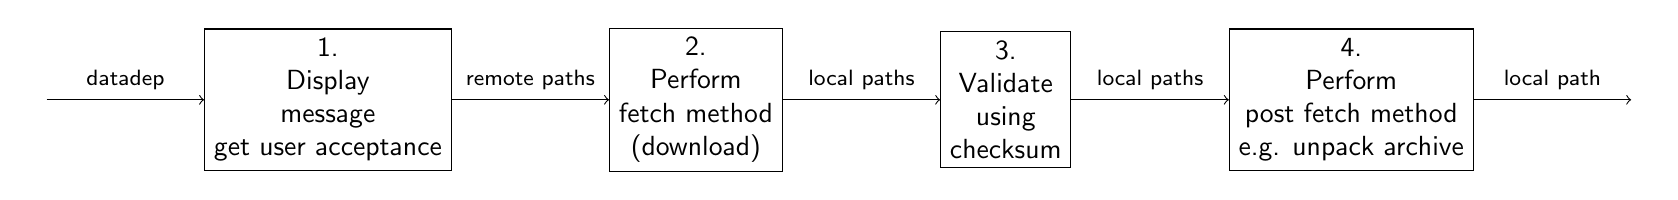
\begin{tikzpicture}[every text node part/.style={align=center}, auto,node distance=2, ->,
							every edge/.append style={every node/.style={font=\footnotesize}}]
			\node(start) {}; 
			\node[draw, rectangle, right= of start] (msg) {1.\\Display\\ message\\ get user acceptance};
			\node[draw, rectangle, right= of msg] (fetch) {2.\\Perform\\ fetch method\\ (download)};
			\node[draw, rectangle, right= of fetch] (checksum) {3.\\Validate\\ using\\ checksum};
			\node[draw, rectangle, right= of checksum] (postfetch) {4.\\Perform \\post fetch method\\ e.g. unpack archive};
			\node[right=of postfetch](end) {};
			
			\path (start)  edge[above] node{datadep}  (msg);
			\path (msg)	edge[above] node{remote paths}  (fetch);
			\path (fetch)	edge[above] node{local paths}  (checksum);
			\path (checksum)	edge[above] node{local paths}  (postfetch);
			\path (postfetch)	edge[above] node{local path}  (end);
		\end{tikzpicture}
	}
	\caption{The core process for resolving a data dependency if a local copy is not found. Each step linked to one of the properties declared in the registration block. \label{fig:retrieve}
	}
\end{figure}


\begin{lstlisting}[frame=single, caption={Example registration block for WordNet. The majority of it is a message for the user.}, label={lst:regblock}] 
  RegisterDataDep("WordNet 3.0",
  """
  Dataset: WordNet 3.0
  Website: https://wordnet.princeton.edu/wordnet

  George A. Miller (1995). 
  WordNet: A Lexical Database for English.
  Communications of the ACM Vol. 38, No. 11: 39-41.

  Christiane Fellbaum (1998, ed.) 
  WordNet: An Electronic Lexical Database. 
  Cambridge, MA: MIT Press.

  License: 
  WordNet Release 3.0 This software and database is 
  being provided to you, the LICENSEE, ... 
  ... and LICENSEE agrees to preserve same.
  """,
  "http://wordnetcode.princeton.edu/3.0/WNdb-3.0.tar.gz",
  "658b1ba191f...f191d2a44e5d25046dc8";
  post_fetch_method = unpack
);
\end{lstlisting}

\subsubsection{Registration Blocks}
The registration block is how a data dependency is described in DataDeps.jl.
It is executable metadata, that when executed returns the data.
Shown in \Cref{lst:regblock} is an example of registration block.
The key information provided in the registration block is:
\begin{description}
\item[name] used to refer to the dependency in code, as in the described \datadep{NAME}
\item[message] the message displayed to the user.
\item[remotepath] a path or a list of paths (normally URLs)to remote copies of the data.
\item[checksum] a checksum (or list of checksums) for the remote files.
\item[fetch_method]  a function  (or list of functions) specifying the method used to download the file, for almost all uses the default \texttt{Base.download} is sufficient.
\item[post_fetch_method] a function  (or list of functions)to call on the fetched files. Most commonly used to unpack an archive.
\end{description}
This properties directly match as the key configurations for the stages shown in \Cref{fig:retrieve}.
When a list of remotepaths is provided,
a the later properties can also be provided as list or individually
The properties after message 


\paragraph{On DOIs}
Every DOI can be used as an URL via the normal \url{http://doi.org/} service.
However, DOIs are often not useful remote paths,
as the DOI specification requires them to redirect to a ``landing page``, rather than to the resource itself.
The landing page will normally contain a link to the resource, often amongst dozens of others.
That resource may not even be on the same domain as the landing page (Indeed the resource may not even be available online, but we are not concerned with those cases.).



\subsubsection{Automating the writing of registration block blocks (DataDepsGenerators.jl)}
Writing a registration block is not complex, however even this can be further automated.
DataDepsGenerators.jl is a package which does this.
In principle it converts metadata of one kind, for example a website describing a dataset,
into another: namely the registration block.




It is important to note that DataDepsGenerators.jl is not to be made a dependency of software that makes use of it.
Rather the code which it generates is added to the software, with a DataDeps.jl dependency.
As DataDepsGenerators.jl makes use of web-scraping and page layout changes much more frequently than URLs,
by repeating the web-scrape in a package every time it loads, that would cause the data dependencies to be unnecessarily fragile.
The registration blocks can be treated as the code, and then regenerated, or manually updated as required by the maintainer.





It is desired that future versions of DataDepsGenerators will leverage the CKAN API (used by data.gov), the Open Access Initiative Protocol for Meta-data Harvesting (OAI-PMH), and other techniques to resolve persistent identifies (such as DOIs), into metadata, and in turn produce the registration blocks.


\subsubsection{Setting up the data, not reading the data (MLDataSets.jl and other packages)}

\subsubsection{Lazy Downloading}


\subsection{Example Workflows}

\subsubsection{Using Existing Datasets}
\begin{enumerate}
	\item Add a data registration block for a dataset
	\item Develop algorithm
	\item Add an additional data registration block for additional dataset 
	\item Develop algorithm
	\item \emph{Repeat as necessary}
	\item Prepare publication
	\item Publish results and software
\end{enumerate}

\subsubsection{Creating Data Along With Software}
This is the work-flow for how an experimental scientist using their software for analysis would use DataDeps.jl.
\begin{enumerate}
	\item Create data store on a web-facing storage provider (either institutional or a service such as DropBox or OwnCloud)
	\item Add the web-facing URL to the data store 
	\item Collect data add it to data store
	\item Delete any local copies of the Data (which may be out of date) to trigger redownloading
	\item Develop analysis script
	\item \emph{Repeat as necessary}
	\item Prepare publication
	\item Transfer data store to a archival storage provider (Eg figshare, datadryad etc. or an institutional repository)
	\item Update data registration block to use new URL, check that the checksum matches.
	\item Publish results and software
\end{enumerate}
Or 
\begin{enumerate}
	\item Add a manual data registration block for the data
	\item Create (locally, or on a mounted network store) the corresponding folder as the data store
	\item Collect data add it to data store
	\item Develop analysis script
	\item \emph{Repeat as necessary}
	\item Prepare publication
	\item Transfer data store to a archival storage provider (Eg figshare, datadryad etc. or an institutional repository)
	\item Update data registration block to use new URL, as an automatic datadep
	\item Publish results and software
\end{enumerate}


This is an exception to DataDeps.jl's assumption that data is public.
For the case of research with concurrent data gathering a publicly available, but secret (https) URL is generally sufficient and works well with DataDeps.jl.
For data which must be truly secured (e.g. medical data) it is theoretically possible to substituted in an a authenticated  download mechanism into DataDeps.jl in the registration block, however this has not been tried in practice.
The other alternative, is the use of a ManualDataDep during development, which functions like a normal automatic DataDep but without the functionality for automatic download, instead the user should manually manage the data.
This allows all the code to be identical except for registration block, which can be changed after the final data is uploaded.



\subsection{Quality Control}

Using AppVeyor and Travis CI testing is automatically performed using the latest stable release of Julia, for the Linux, Windows, and Mac environments.
The DataDeps.jl tests include unit tests of key components, as well as comprehensive system/integration tests of different configurations of data dependencies.
These latter tests also form high quality examples to supplement the documentation for users to looking to see how to use the package.
The user can trigger these tests to ensure everything is working on their local machine by the standard julia mechanism: running \texttt{Pkg.test(``DataDeps'')} respectively.


The primary mechanism for user feedback is via Github issues on the repository.
Bugs and feature requests, even purely by the authors, are tracked using the Github issues.

\section{Availability}
\subsection{Operating system}
DataDeps.jl is verified to work on Windows 7+, Linux, Mac OSX.

\subsection{Programming language}
Julia v0.6

\subsection{Dependencies}
DataDeps.jl has been careful designed to minimise dependencies so as to maximise its usability without requiring the installation of many packages.
Adding it to a package thus does not substantially increase time taken to install the package.
It is currently only dependent on SHA.jl for the default generation and checking of checksums.

\section*{List of contributors}

\textcolor{blue}{Please list anyone who helped to create the software (who may also not be an author of this paper), including their roles and affiliations.}

\subsection{Software location:}

{\bf Archive} \textcolor{blue}{(e.g. institutional repository, general repository) (required – please see instructions on journal website for depositing archive copy of software in a suitable repository)} 

\begin{description}[noitemsep,topsep=0pt]
	\item[Name:] \textcolor{blue}{The name of the archive.}
	\item[Persistent identifier:] \textcolor{blue}{e.g. DOI, handle, PURL, etc.}
	\item[Licence:] \textcolor{blue}{Open license under which the software is licensed.}
	\item[Publisher:]  \textcolor{blue}{Name of the person who deposited the software.}
	\item[Version published:] \textcolor{blue}{The version number of the software archived.}
	\item[Date published:] \textcolor{blue}{dd/mm/yy}
\end{description}



{\bf Code repository} GitHub

\begin{description}[noitemsep,topsep=0pt]
	\item[Name:] oxinabox/DataDeps.jl
	\item[Persistent identifier:] \url{https://github.com/oxinabox/DataDeps.jl/blob/master/README.md}
	\item[Licence:] MIT
	\item[Date published:] 28/11/2017
\end{description}


\subsection{Language}
English.

\section{Reuse potential}
\textcolor{blue}{Please describe in as much detail as possible the ways in which the software could be reused by other researchers both within and outside of your field. This should include the use cases for the software, and also details of how the software might be modified or extended (including how contributors should contact you) if appropriate. Also you must include details of what support mechanisms are in place for this software (even if there is no support).}

As a purely supporting library, without contribution of its own, DataDeps.jl exists only to be reused.
The cases in which is should be reused are well discussed above.
It is of benefit to any research tool, or scientific script that has a dependency on data for it's functioning or for generation of its result.


DataDeps.jl is extendible via the normal julia methods of subtyping, and composition.
Additional kinds of \texttt{DataDep} can be created, for example to add an additional validation step,
while still reusing the behaviour defined.
Such new types can be created in their own packages, or contributed to the open source DataDeps.jl package.


Julia is a relatively new language with a rapidly growing ecosystem of packages.
It is seeing a lot of up take in many fields of computation sciences, data science and other technical computing.
By establishing tools like DataDeps.jl now, which support the easy reuse of code,
we hope to promote greater resolvability of packages being created later.
Thus in turn leading to more reproducible data and computational science in the future.

\section*{Acknowledgements}
Thank to Christof Stocker, the creator of MLDatasets.jl (and numerous other packages), in particular for his bug reports, feature requests and code reviews; and for the initial discussion leading to the creation of this tool.
\pdfcomment{Maybe should make Christof a coauthor?}

\section*{Funding statement}

\textcolor{blue}{If the software resulted from funded research please give the funder and grant number.}

\section*{Competing interests}
The authors declare that they have no competing interests.

\section*{References}

\textcolor{blue}{Please enter references in the Harvard style and include a DOI where available, citing them in the text with a number in square brackets, e.g. \\ }

\printbibliography

\vspace{2cm}

\rule{\textwidth}{1pt}

{ \bf Copyright Notice} \\
Authors who publish with this journal agree to the following terms: \\

Authors retain copyright and grant the journal right of first publication with the work simultaneously licensed under a  \href{http://creativecommons.org/licenses/by/3.0/}{Creative Commons Attribution License} that allows others to share the work with an acknowledgement of the work's authorship and initial publication in this journal. \\

Authors are able to enter into separate, additional contractual arrangements for the non-exclusive distribution of the journal's published version of the work (e.g., post it to an institutional repository or publish it in a book), with an acknowledgement of its initial publication in this journal. \\

By submitting this paper you agree to the terms of this Copyright Notice, which will apply to this submission if and when it is published by this journal.


\end{document}
